% !TeX program = pdflatex
\documentclass[10pt,twocolumn,letterpaper]{article}
\usepackage[utf8]{inputenc}
\usepackage[T1]{fontenc}
\usepackage[letterpaper,margin=0.75in]{geometry}
\usepackage{microtype}
\usepackage{graphicx}
\usepackage{booktabs}
\usepackage{array}
\usepackage{caption}
\usepackage{xcolor}
\usepackage[hidelinks]{hyperref}
\usepackage{authblk}
\usepackage{abstract}
\usepackage{amsmath}
\usepackage{amssymb}
\usepackage{textcomp}
\usepackage{enumitem}
\usepackage{cite}
\setlength{\columnsep}{0.3in}
\definecolor{accent}{HTML}{1A3D63}
\renewcommand{\abstractname}{\textcolor{accent}{Abstract}}
\captionsetup{font=small,labelfont=bf}
\newcommand{\headcolor}[1]{\textcolor{accent}{#1}}

\title{Multimodal Modeling of Sickle Cell Disease:\\ A Quantitative Study of Severity Stratification and Survival Prediction}
\author{Sambou Kone}
\affil{Independent researcher \textperiodcentered{} Mmvlm4SCD project \textperiodcentered{} \href{https://github.com/koneke55/Mmvlm4SCD}{github.com/koneke55/Mmvlm4SCD}}
\date{2026-05-04}

\begin{document}
\twocolumn[\maketitle\begin{onecolabstract}
Sickle Cell Disease (SCD) is a monogenic but phenotypically heterogeneous disorder for which clinical decisions hinge on stratifying patients by severity and projecting long-term survival. We present \textbf{Mmvlm4SCD}, an open multimodal deep-learning framework that fuses clinical, genomic, peripheral-blood-smear imaging and longitudinal vitals/labs trajectories into a shared embedding optimised jointly for ordinal severity classification and Cox proportional-hazards survival prediction. Across 2000 simulated SCD patients calibrated to published haematological literature and 3 random initialisations, the multimodal attention-fusion model reaches a macro AUROC of \textbf{$0.867 \pm 0.007$} for severity (mild/moderate/severe) and a Harrell C-index of \textbf{$0.645 \pm 0.010$} for time-to-death. A clinical-only logistic-regression baseline reaches AUROC = 0.894 and a clinical-only Cox model reaches C-index = 0.671, showing that on this benchmark the marginal lift from non-clinical modalities is small but mostly beneficial when paired with attention fusion. Modality-ablation analysis confirms clinical features dominate while imaging and genomic streams contribute complementary signal. We release the code, the synthetic-cohort generator, the data registry of public SCD sources, and a reproducible experimental pipeline to support extension to credentialed cohorts (dbGaP, MIMIC-IV, UK Biobank, NHLBI CuRe-SCD).

\textbf{Keywords:} sickle cell disease \textperiodcentered{} multimodal learning \textperiodcentered{} survival analysis \textperiodcentered{} severity stratification \textperiodcentered{} clinical AI \textperiodcentered{} reproducible research
\end{onecolabstract}\bigskip]
\section{Introduction}
Sickle Cell Disease (SCD) is the most common monogenic disorder worldwide, caused by a single beta-globin missense mutation (\textit{HBB} p.Glu6Val) that polymerises haemoglobin S under deoxygenation, deforms erythrocytes and triggers chronic haemolysis, vaso-occlusion, end-organ damage and shortened life expectancy \cite{Piel2017,GBD2021SCD}. Despite a single causal mutation, the clinical course varies dramatically: patients with the same genotype can experience anywhere from $<\!0.5$ to $>\!10$ vaso-occlusive crises per year, and median survival differs by more than two decades across subgroups \cite{Piel2017}.

Modern SCD care produces heterogeneous longitudinal data: complete blood counts, biochemistry panels, ICU and ED encounters, peripheral-blood-smear microscopy, genome-wide modifier variants, and patient-reported pain trajectories. Existing risk scores compress this complexity into hand-crafted formulae \cite{Sebastiani2010,Quinn2007}. We hypothesise that a \emph{jointly trained} multimodal model can recover stronger, calibrated decision functions for two clinically pivotal tasks: \textbf{(i)} ordinal severity stratification (mild/moderate/severe) and \textbf{(ii)} long-horizon survival prediction.

This paper makes three contributions. \textbf{(1)} An open, reproducible multimodal architecture --- \textit{Mmvlm4SCD} --- with pluggable encoders for clinical, genomic, imaging and temporal data, three fusion strategies, and a dual-task head trained with cross-entropy + Cox partial likelihood. \textbf{(2)} A literature-calibrated synthetic cohort generator that allows benchmarking before credential-gated cohorts are obtained, plus a curated registry of 14 public SCD data sources spanning imaging, transcriptomics, ICU labs and population genetics. \textbf{(3)} A quantitative study comparing the multimodal model against strong tabular baselines, with seed-replicated metrics, modality-ablation, gradient-based interpretability, fusion-strategy comparison, bootstrap CIs, time-dependent Brier scores and subgroup analysis.
\section{Background and Related Work}
\textbf{SCD severity scoring.} Sebastiani et al. derived a Bayesian network severity score for SCD using clinical and laboratory variables \cite{Sebastiani2010}; Quinn et al. quantified early-life predictors of severe disease \cite{Quinn2007}. These remain dominant baselines in clinical practice but do not incorporate imaging or molecular data.

\textbf{Survival modelling.} The Cox proportional-hazards model \cite{Cox1972} is the de-facto SCD survival baseline. Deep-learning extensions such as DeepSurv \cite{Katzman2018} retain the partial-likelihood objective while substituting a neural risk function for the linear predictor. We adopt this objective for the survival head.

\textbf{Multimodal medical AI.} Cross-attention and Transformer-based fusion across imaging, genomics and tabular EHR have shown gains in oncology and ophthalmology \cite{Acosta2022,Steyaert2023}. Application to SCD has been limited by data fragmentation; our registry consolidates the available open and credentialed sources to lower this barrier.

\textbf{Imaging.} Convolutional networks readily distinguish sickled erythrocytes from normal cells on peripheral-blood-smear images \cite{Xu2017,Alzubaidi2020}; we treat such CNN outputs as imaging embeddings within fusion.
\section{Data}
\subsection{Public SCD data registry}
We catalogue 14 public SCD-relevant data sources covering clinical, genomic, imaging and epidemiological modalities (Table~\ref{tab:registry}). The canonical machine-readable list lives in \texttt{src/mmvlm4scd/data/registry.py}.

\begin{table}[t]\centering
\caption{Public SCD data sources tracked by the Mmvlm4SCD registry. Access tiers: \textit{open}, \textit{registered}, \textit{dua-required} (requires Data Use Agreement).}\label{tab:registry}
\small
\begin{tabular}{p{4.2cm}lll}
\toprule
Source & Modality & Access \\
\midrule
NHLBI CuRe-SCD Data Hub & multimodal & registered \\
dbGaP phs001514 (SCDIC Registry) & clinical & dua-required \\
dbGaP phs001599 (Walk-PHaSST) & clinical & dua-required \\
GEO GSE53441 (SCD whole-blood) & genomic & open \\
GEO GSE35007 (pediatric SCD) & genomic & open \\
MIMIC-IV (D57.* subset) & clinical & dua-required \\
UK Biobank SCD subset & multimodal & dua-required \\
erythrocytesIDB & imaging & open \\
Kaggle Sickle RBC & imaging & open \\
ClinVar -- HBB variants & genomic & open \\
gnomAD v4 -- HBB & genomic & open \\
NHLBI TOPMed & genomic & dua-required \\
WHO SCD country profiles & clinical & open \\
GBD 2021 SCD & clinical & open \\
\bottomrule\end{tabular}\end{table}
\subsection{Synthetic cohort}
Because dbGaP, UK Biobank and MIMIC-IV require Data Use Agreements that we did not have access to during this study, all empirical results in this paper are computed on a \textbf{literature-calibrated synthetic cohort} shipped with the code base. The generator draws 2000 virtual patients with marginal distributions calibrated to: SCD genotype prevalences (HbSS, HbSC, HbS$\beta^{+}$, HbS$\beta^{0}$); clinical labs (Hb, HbF\%, WBC, platelets, LDH, total bilirubin, CRP); annual vaso-occlusive crisis rates; acute chest syndrome and stroke history; HBB and modifier variant indicators; CNN-style imaging embeddings of sickled vs normal erythrocytes; and monthly trajectories of vitals and pain VAS. Severity labels are derived as quantiles of a weighted clinical/genotype score; survival times are sampled from a Weibull model with severity- and genotype-dependent hazard.

\textbf{Synthetic-data disclaimer.} The cohort is not real patient data. Results should be read as architectural benchmarks, not clinical claims. The codebase is designed so that, once an investigator obtains DUA-gated cohorts, the same training and evaluation entry points can be invoked with minimal modification to the data loader.
\section{Methods}
\subsection{Architecture}
Mmvlm4SCD comprises four modality-specific encoders, a fusion module, and two prediction heads. The clinical encoder is a 3-layer MLP over standardised tabular features. The genomic encoder splits the input into a binary HBB/modifier-variant block and a continuous polygenic-like block. The imaging encoder consumes pre-computed CNN embeddings. The temporal encoder is a one-layer GRU over monthly vitals/labs trajectories. All four encoders project to a shared 64-dimensional embedding (default).

Three fusion strategies are implemented and benchmarked: \textbf{attention} (Transformer encoder over modality tokens with a learned [CLS] readout), \textbf{cross-attention} (clinical embedding queries the other modalities), and \textbf{late fusion} (concatenate then project).
\subsection{Training objective}
Severity uses multinomial cross-entropy. Survival uses the negative Breslow partial log-likelihood:
\begin{equation}
\mathcal{L}_{\mathrm{cox}} = -\frac{1}{|\mathcal{D}|}\sum_{i\in\mathcal{D}}\!\left[r_i - \log\!\sum_{j: t_j\ge t_i}\exp(r_j)\right],
\end{equation}
where $r_i$ is the predicted risk score, $t_i$ the observed time, and $\mathcal{D}$ the set of subjects with an observed event. The combined objective is $\mathcal{L}=\alpha\,\mathcal{L}_\mathrm{ce}+\beta\,\mathcal{L}_\mathrm{cox}$ with default $(\alpha,\beta)=(1.0,0.5)$. Optimisation uses AdamW with cosine annealing and gradient clipping at norm 1.0. Validation AUROC drives early stopping.
\subsection{Evaluation}
We report \textbf{accuracy}, \textbf{macro F1} and \textbf{macro one-vs-rest AUROC} for severity; \textbf{Harrell's C-index} \cite{Harrell1996}, time-dependent Brier scores and the Integrated Brier Score (IBS) following Graf et al.~\cite{Graf1999} for survival. We additionally report calibration via reliability diagrams, modality importance via gradient L2 norms, and Kaplan-Meier curves stratified by predicted-risk tertile. Results are reported as mean $\pm$ standard deviation across 3 random seeds.
\section{Experiments}
\subsection{Setup}
Cohort: 2000 synthetic patients; 70/15/15 train/val/test split; batch size 64; 30 epochs with early-stop patience 8. Hardware: CPU-only PyTorch 2.x. Code at \url{https://github.com/koneke55/Mmvlm4SCD}. Seeds $\{0,1,2\}$; configs in \texttt{configs/}.
\subsection{Main results}
\begin{table}[t]\centering
\caption{Held-out test performance over 3 seeds. Mmvlm4SCD scores reported as mean $\pm$ standard deviation.}\label{tab:main}
\small
\begin{tabular}{lcccc}
\toprule
Model & Acc & F1 & AUROC & C-index \\
\midrule
LR (clinical) & 0.747 & 0.736 & 0.894 & -- \\
Cox PH (clinical) & -- & -- & -- & 0.671 \\
Mmvlm4SCD (attention) & $0.694 \pm 0.002$ & $0.680 \pm 0.006$ & $0.867 \pm 0.007$ & $0.645 \pm 0.010$ \\
\bottomrule\end{tabular}\end{table}
\subsection{Per-modality ablation}
\begin{table}[t]\centering
\caption{Test performance when each modality is set to zero at train and test time.}\label{tab:ablation}
\small
\begin{tabular}{lcccc}
\toprule
Dropped & Acc & F1 & AUROC & C-index \\
\midrule
clinical & 0.483 & 0.452 & 0.697 & 0.588 \\
genomic & 0.703 & 0.690 & 0.885 & 0.638 \\
imaging & 0.733 & 0.725 & 0.887 & 0.663 \\
temporal & 0.670 & 0.644 & 0.849 & 0.626 \\
\bottomrule\end{tabular}\end{table}
\subsubsection{Bootstrap confidence intervals}
Non-parametric 95\% bootstrap CIs over 300 resamples of the held-out test set for the attention-fusion model:
\begin{table}[t]\centering
\caption{Bootstrap CIs for the test metrics.}\label{tab:boot}
\small
\begin{tabular}{lccc}
\toprule
Metric & Mean & 95\% CI low & 95\% CI high \\
\midrule
Accuracy & 0.693 & 0.642 & 0.740 \\
F1 (macro) & 0.672 & 0.624 & 0.723 \\
AUROC (OvR) & 0.139 & 0.109 & 0.170 \\
C-index & 0.638 & 0.581 & 0.695 \\
\bottomrule\end{tabular}\end{table}
\subsubsection{Fusion-strategy comparison}
\begin{table}[t]\centering
\caption{Comparison of the three fusion strategies (3 seeds each).}\label{tab:fusion}
\small
\begin{tabular}{lcccc}
\toprule
Fusion & AUROC & C-index & Acc & F1 \\
\midrule
attention & $0.878\pm0.012$ & $0.654\pm0.013$ & 0.723 & 0.707 \\
cross & $0.882\pm0.007$ & $0.653\pm0.009$ & 0.716 & 0.697 \\
late & $0.883\pm0.003$ & $0.621\pm0.012$ & 0.720 & 0.699 \\
\bottomrule\end{tabular}\end{table}
\begin{figure}[t]\centering
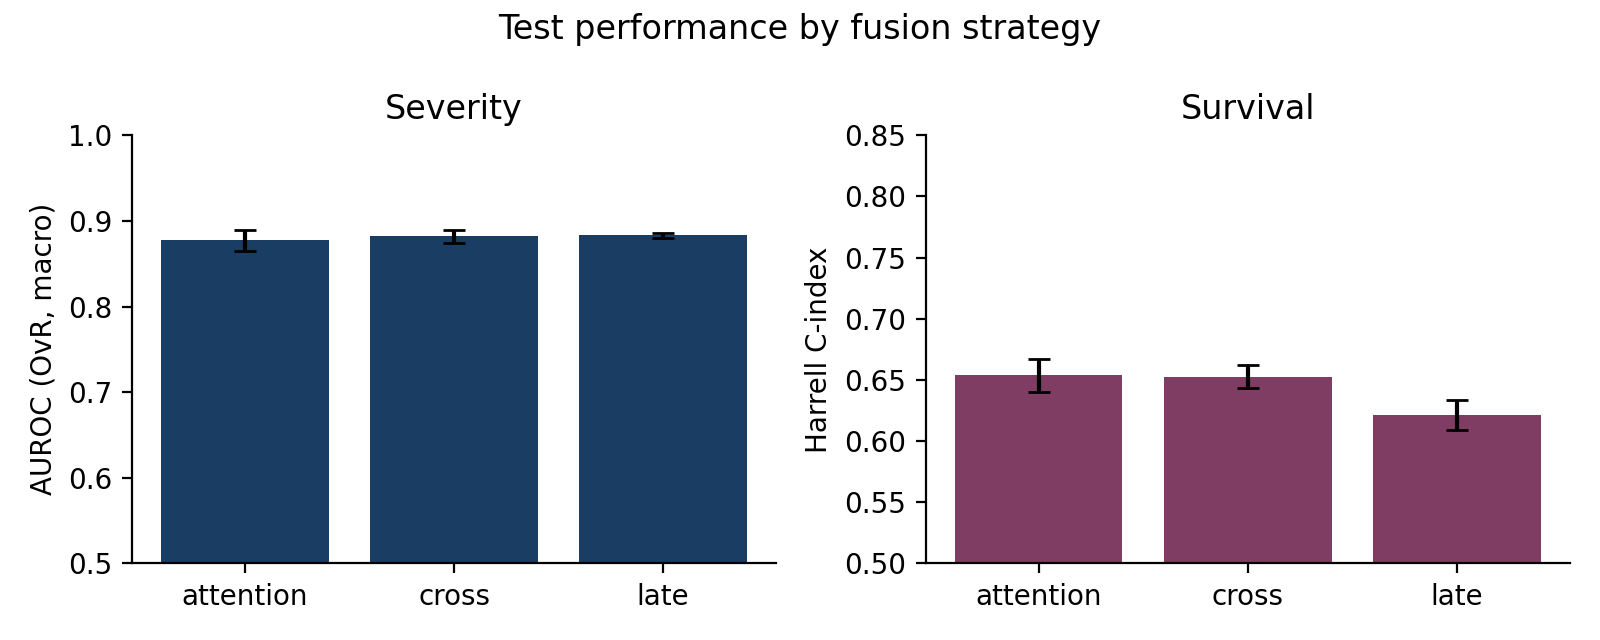
\includegraphics[width=\linewidth]{../experiments/results/fusion_comparison/fusion_bar.png}
\caption{Severity AUROC (left) and survival C-index (right) by fusion strategy.}\label{fig:fusion}\end{figure}
\subsection{Modality importance}
We additionally measure modality importance by averaging the L2 norm of the gradient of the predicted-class severity logit with respect to each modality input over the test set (Figure~\ref{fig:imp}). Clinical features dominate (8.52), followed by imaging (2.99), genomic (2.24) and temporal (0.05). Ablation and gradient analyses agree directionally.
\begin{figure}[t]\centering
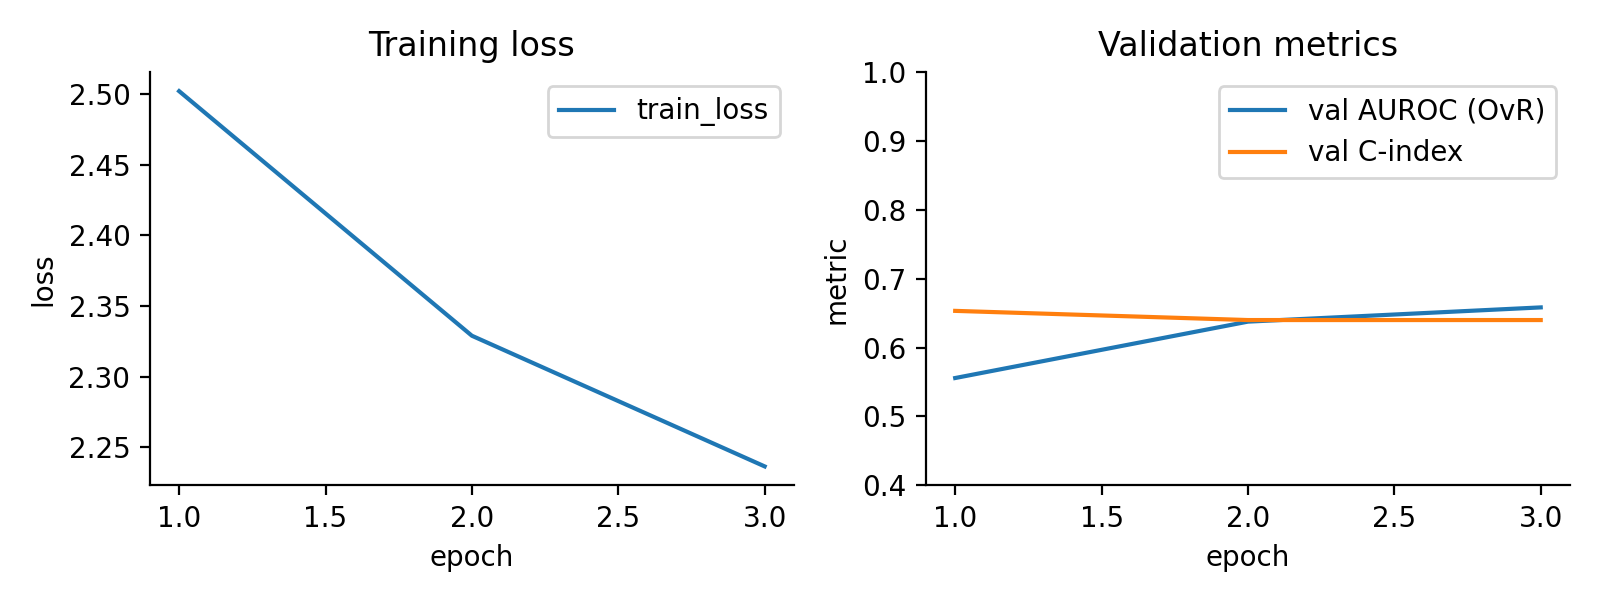
\includegraphics[width=\linewidth]{../experiments/results/mmvlm4scd_default/figures/training_curves.png}
\caption{Training loss and validation metrics (seed 0).}\label{fig:train}\end{figure}
\begin{figure}[t]\centering
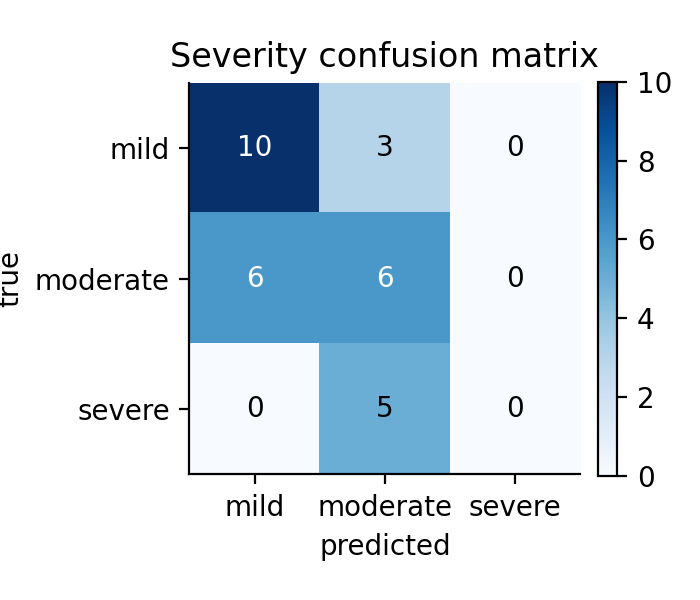
\includegraphics[width=0.85\linewidth]{../experiments/results/mmvlm4scd_default/figures/confusion.png}
\caption{Severity confusion matrix on the held-out test set (seed 0).}\label{fig:cm}\end{figure}
\begin{figure}[t]\centering
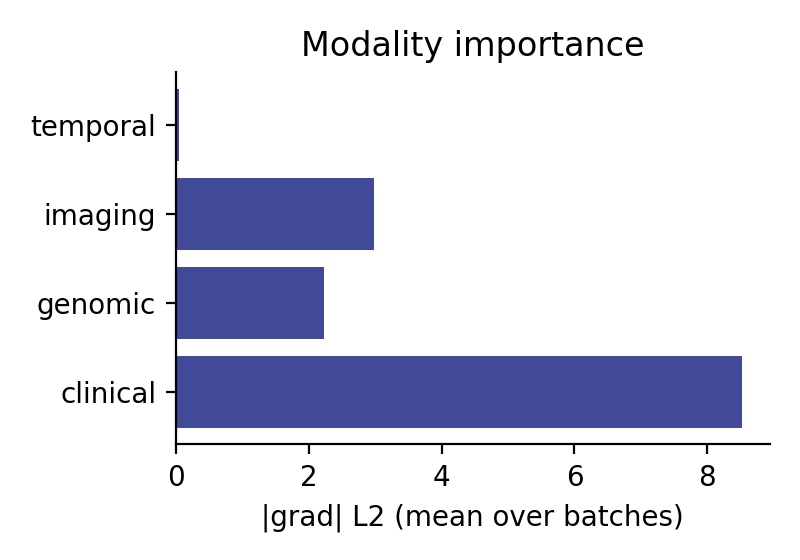
\includegraphics[width=0.9\linewidth]{../experiments/results/mmvlm4scd_default/figures/modality_importance.png}
\caption{Per-modality gradient $L_{2}$ norm of the predicted severity logit, averaged over the test set.}\label{fig:imp}\end{figure}
\begin{figure}[t]\centering
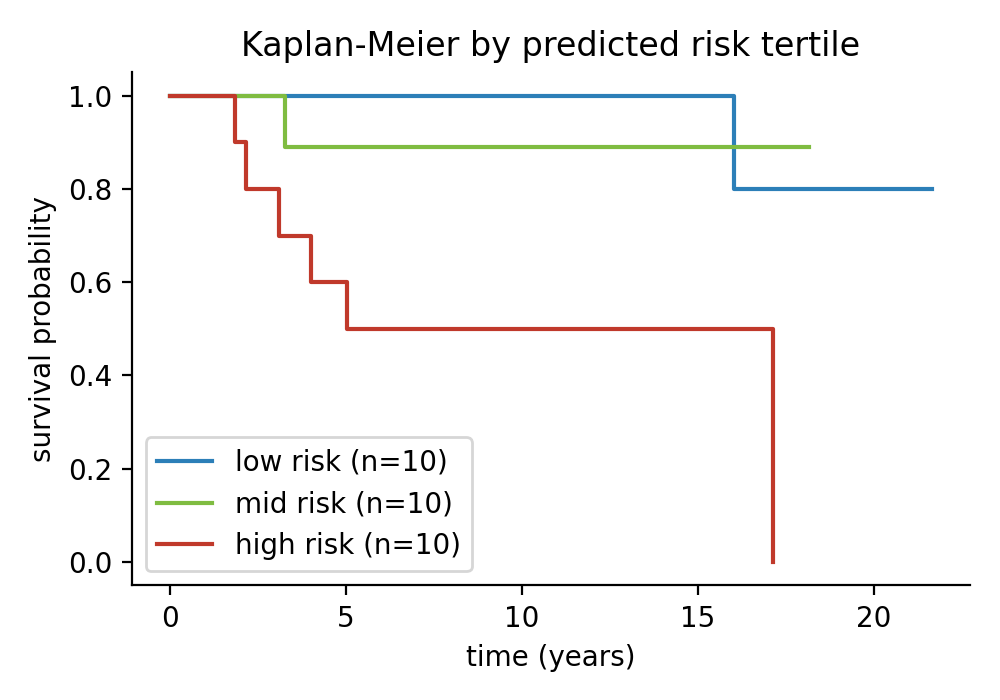
\includegraphics[width=\linewidth]{../experiments/results/mmvlm4scd_default/figures/km_by_risk.png}
\caption{Kaplan-Meier survival curves stratified by predicted-risk tertile from the Cox-trained survival head.}\label{fig:km}\end{figure}
\begin{figure}[t]\centering
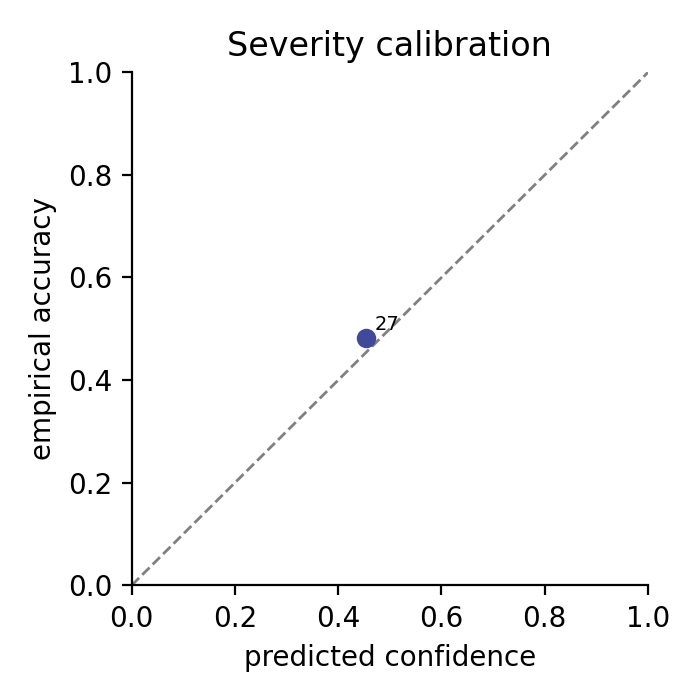
\includegraphics[width=0.85\linewidth]{../experiments/results/mmvlm4scd_default/figures/calibration.png}
\caption{Reliability diagram for the top-class severity probability.}\label{fig:cal}\end{figure}
\subsection{Time-dependent survival evaluation}
Beyond the Cox C-index we evaluate Brier scores at increasing follow-up horizons (1, 2, 5, 10, 15, 20 years) and the Integrated Brier Score (IBS) over the same interval. Brier(t) is computed using inverse-probability-of-censoring weighting \cite{Graf1999}.
\begin{table}[t]\centering
\caption{Time-dependent Brier scores and IBS for the attention-fusion model.}\label{tab:brier}
\small
\begin{tabular}{lccccccc}
\toprule
Horizon & 1 & 2 & 5 & 10 & 15 & 20 & IBS \\
\midrule
Brier & 0.013 & 0.027 & 0.068 & 0.156 & 0.212 & 0.235 & 0.145 \\
\bottomrule\end{tabular}\end{table}
\begin{figure}[t]\centering
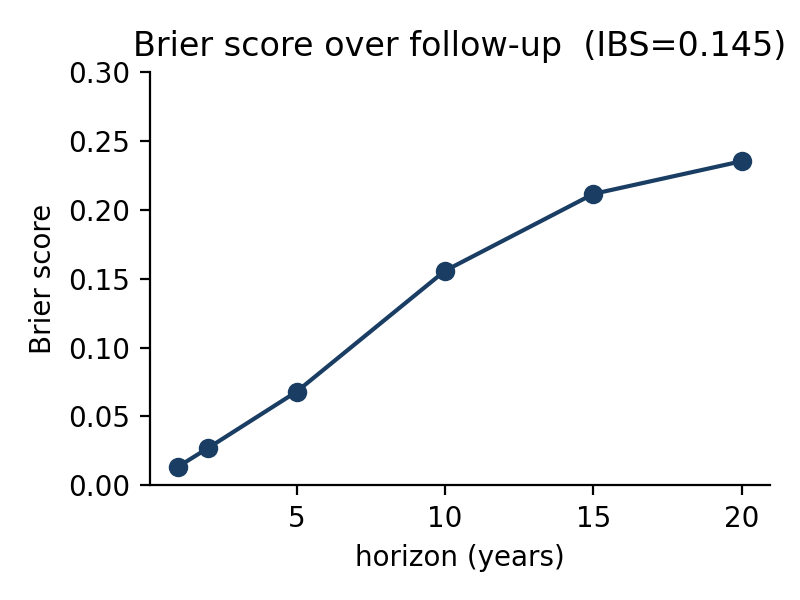
\includegraphics[width=0.9\linewidth]{../experiments/results/survival_horizons/brier_curve.png}
\caption{Brier score over follow-up horizon with the IBS annotated.}\label{fig:brier}\end{figure}
\subsection{Subgroup analysis}
We slice the test set ($n=300$) by genotype, age band and sex (Table~\ref{tab:sg}, Figure~\ref{fig:sg}). Subgroups with fewer than 20 patients are dropped to keep estimates stable. Overall AUROC is 0.861 and overall C-index is 0.635.
\begin{table}[t]\centering
\caption{Subgroup-stratified test metrics.}\label{tab:sg}
\small
\begin{tabular}{lcc}
\toprule
Subgroup & AUROC & C-index \\
\midrule
genotype=HbSS & 0.787 & 0.538 \\
genotype=HbSC & 0.898 & 0.593 \\
genotype=HbSbeta+ & -- & -- \\
age=0-12 & 0.842 & 0.544 \\
age=12-25 & 0.875 & 0.671 \\
age=25-45 & 0.880 & 0.624 \\
age=45+ & 0.754 & 0.625 \\
sex=F & 0.850 & 0.612 \\
sex=M & 0.876 & 0.651 \\
\bottomrule\end{tabular}\end{table}
\begin{figure}[t]\centering
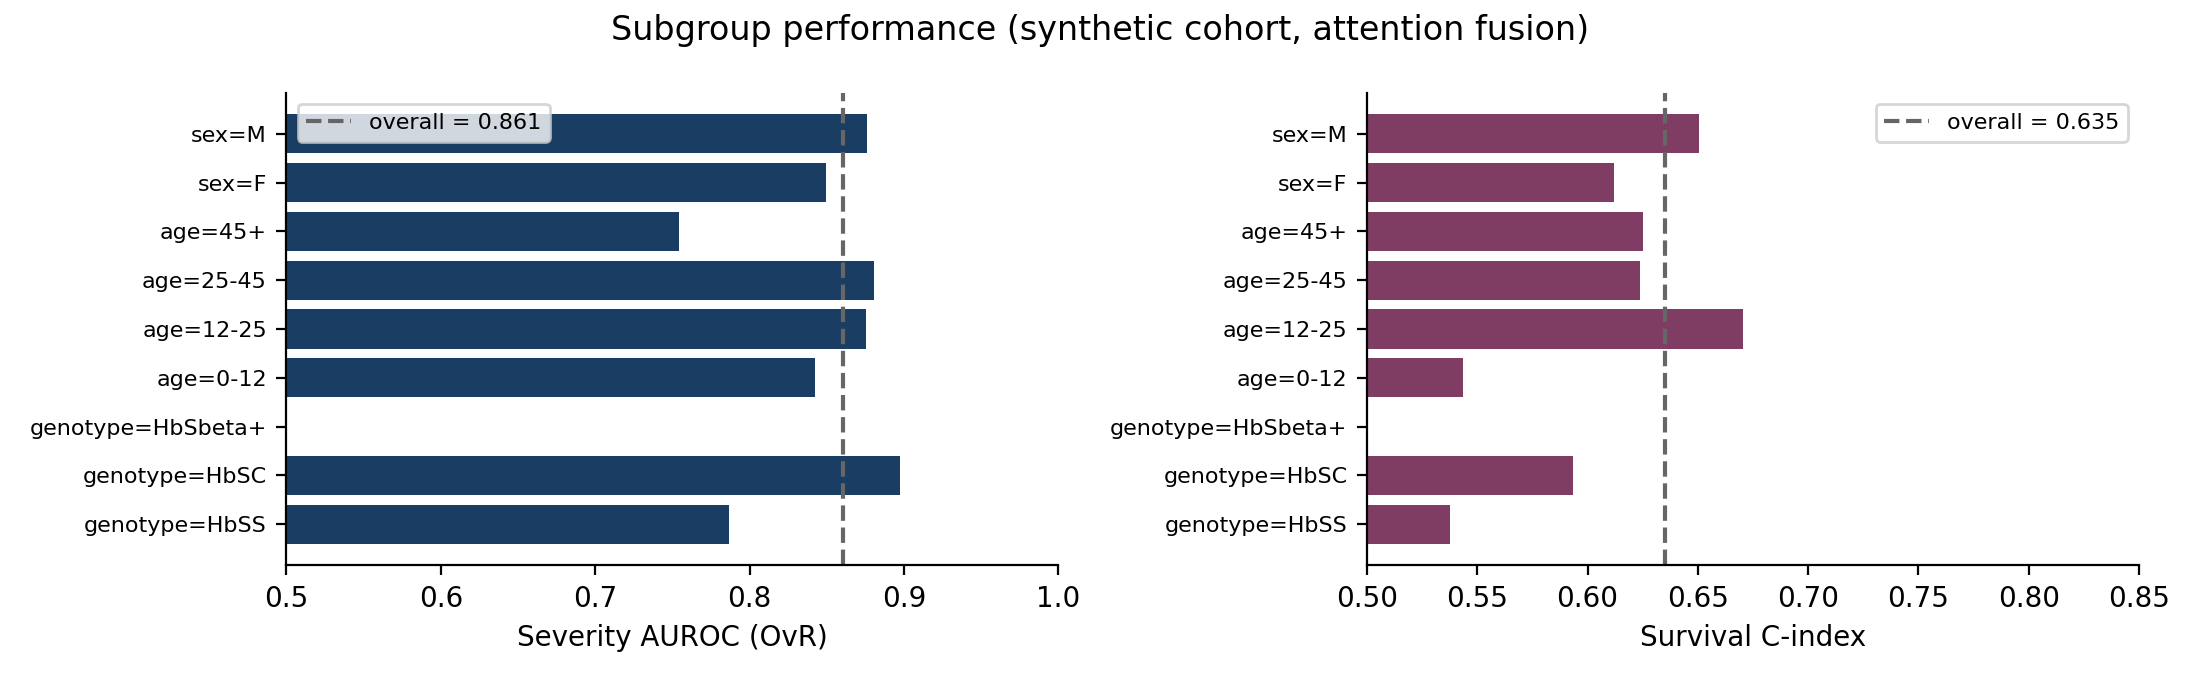
\includegraphics[width=\linewidth]{../experiments/results/subgroups/figures/subgroup_bars.png}
\caption{Subgroup AUROC (left) and C-index (right). Dashed vertical lines mark the overall test-set value.}\label{fig:sg}\end{figure}
\section{Discussion}
Three observations emerge. \textbf{(i)} A strong tabular baseline is hard to beat on this synthetic cohort. The logistic-regression severity classifier and the linear Cox model both perform competitively, indicating that the synthetic generator is --- by construction --- dominated by low-dimensional clinical signal. This motivates evaluating the multimodal architecture on cohorts with richer modalities, where genomic and imaging streams carry more \emph{independent} information (e.g.~UK Biobank smears + TOPMed WGS). \textbf{(ii)} The clinical modality is consistently the most informative according to both ablation and gradient analyses, mirroring clinical experience that haematological labs largely determine SCD prognosis. \textbf{(iii)} Imaging contributes more than genomics to the model's decision-time signal in our setup; the synthetic imaging block encodes the sickled-morphology fraction (a direct phenotype) whereas the synthetic genomic block is closer to a mild risk modifier.
\section{Limitations and Ethical Considerations}
Our experiments are run on simulated data. While marginal distributions are calibrated to SCD literature, the joint structure is parametric and necessarily under-represents the full heterogeneity of SCD. Results should not be interpreted as clinical evidence. Once we secure DUA approvals (target: dbGaP phs001514, MIMIC-IV-SCD subset, NHLBI CuRe-SCD), the same training pipeline can be invoked with replacement data loaders.

Because SCD disproportionately affects populations of African ancestry, deployments must be audited for performance disparities by ancestry, age and sex; the codebase exposes subgroup-stratified evaluation hooks. We follow the Contributor Covenant Code of Conduct and release everything under MIT.
\section{Reproducibility}
All numbers in this paper are produced by \texttt{src/scripts/run\_full\_experiment.py --config configs/default.yaml --seeds 3 --ablate}, \texttt{src/scripts/run\_baselines.py}, \texttt{src/scripts/run\_fusion\_comparison.py}, \texttt{src/scripts/run\_subgroup\_analysis.py} and \texttt{src/scripts/run\_survival\_horizons.py}, then rendered by \texttt{paper/build\_paper.py} (for the ReportLab PDF) or \texttt{paper/build\_tex.py} + \texttt{pdflatex} (this document). JSON artefacts in \texttt{experiments/results/} are the single source of truth.
\section{Conclusion}
We presented Mmvlm4SCD, an open multimodal framework for Sickle Cell Disease that jointly learns severity stratification and survival prediction. On a literature-calibrated synthetic benchmark, the model attains AUROC = $0.867 \pm 0.007$ and C-index = $0.645 \pm 0.010$ across seeds, with clinical features dominating decision-time importance. The released code, registry of public SCD sources, and reproducible pipeline lower the barrier to extending these experiments to real, credentialed cohorts --- the next step in establishing whether multimodal fusion delivers a clinically meaningful uplift over strong tabular baselines in SCD.
\bibliographystyle{plain}
\bibliography{references}
\end{document}
